\maketitle

\section{situation}
\begin{frame}
  \frametitle{the cool kids are using overleaf these days}
  \begin{itemize}
    \item[{\DejaSans ✓}] edit LaTeX documents in the webbrowser 
    \item[{\DejaSans ✓}] be collaborative with multiple users editing the same document
    \item[{\DejaSans ✓}] automatic rebuild and pdf view
    \item[{\DejaSans ✓}] version control
    \item[{\DejaSans ✓}] all in the cloud
    \item<2->[{\DejaSans ☹}] not much of a choice, manager starts with one tool and the rest has to join
      \newline (when collaborating, you have to agree on something anyway)
    \item<2->[{\DejaSans ☺}] one of the least disappointing vim binding implementations in a browser I've worked with
    \item<2->[{\DejaSans ☹}] all local plugins and settings inaccessible
    \item<2->[{\DejaSans ☹}] no command line tools
    \item<3->[{\DejaSans 😃}] synchronised \texttt{git} access!
  \end{itemize}
\end{frame}

\begin{frame}[t]
  \frametitle{discussions are in place}
  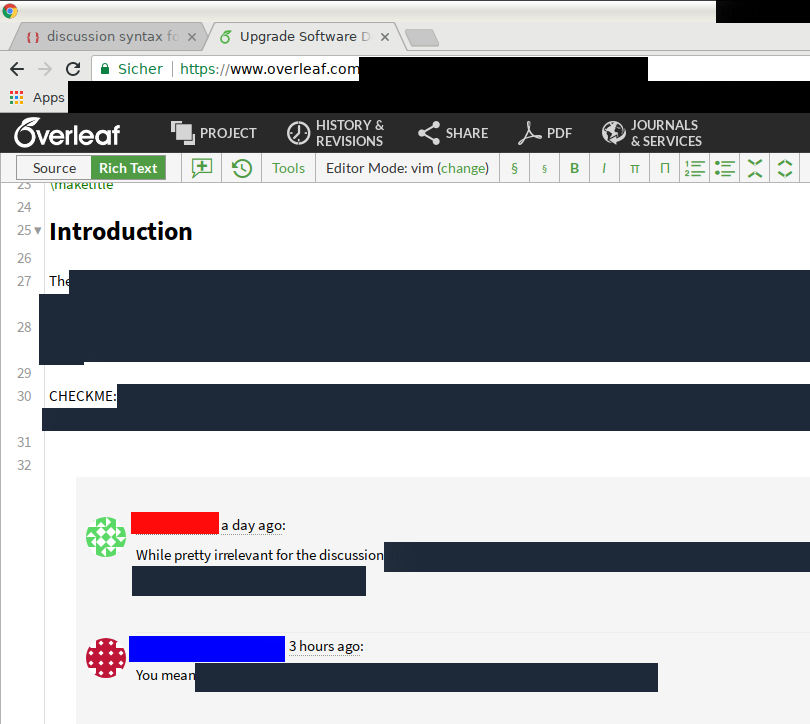
\includegraphics[height=.95\textheight]{./discuss_wysiwyg.png}

  \only<2>{
    \vspace{-.5\textheight}
    \begin{block}{Discussions kept in TeX comments}
      {\DejaSans ✓} discussions accessible through \texttt{git}

      {\DejaSans ✘} but \dots only really nice in the WYSIWYG view
    \end{block}
  }

\end{frame}

\section{problem}
\begin{frame}[t,fragile]
  \frametitle{discussions are error prone}
  \begin{lstlisting}[language=tex,gobble=2]
  % * <email@server.tld> 2018-02-05T14:56:52.585Z:
  %
  % I would phrase this similar ...
  %
  % ^ <other.email@server.tld> 2018-02-12T14:05:57.936Z:
  %
  % I agree, I just wanted to make it clear that I think this is a very hard problem.
  %
  % ^.
  \end{lstlisting}

  \begin{block}{only comments in the correct syntax get rendered}
    It happened to us multiple times that responses written in the source view in the browser were not seen byall users.
  \end{block}
  \only<2>{
    \vspace{-.6\textheight}
    \begin{alertblock}{That will happen again}
      \begin{itemize}
        \item if someone uses the page with default settings we can hardly blame them
        \item \dots maybe enforce WYSIWYG through non-technical means
      \end{itemize}
    \end{alertblock}
  }
  \only<3>{
    \vspace{-.6\textheight}
    \begin{exampleblock}{But maybe help where the issue is known}
      \begin{itemize}
        \item Getting the syntax right is easy for a computer
        \item[$\Rightarrow$] Let the computer do the job
      \end{itemize}
    \end{exampleblock}
  }

\end{frame}

\section{solution}
\begin{frame}
  \frametitle{I have something for you}
  \begin{block}{what's there}
    \begin{itemize}
      \item code on \myhref{https://github.com/pseyfert/overleaf-commenter}{https://github.com/pseyfert/overleaf-commenter}.
      \item mostly python for printing to the command line
      \item rudimentary vim plugin integration
        \begin{itemize}
          \item insert after cursor
          \item check if discussion already present (yes: reply, no: start)
        \end{itemize}
      \item code under AGPL, copyright with my employer
    \end{itemize}
  \end{block}
  \begin{exampleblock}{I'd be happy if this is of use for somebody}
    \begin{itemize}
      \item I'll be happy to merge a pull request with emacs integration
    \end{itemize}
  \end{exampleblock}
\end{frame}
\begin{frame}
  \frametitle{future developments}
  \begin{itemize}
    \item I tried overleaf v2 very early in the test phase
    \item direct \texttt{git} access is gone (only git\emph{hub} export/import)
      \begin{itemize}
        \item but overleaf says they're working on bringing it back
      \end{itemize}
    \item discussions not taking place in tex comments anymore
      \begin{itemize}
        \item[{\DejaSans ☹}] \texttt{overleaf-commenter} might become useless
        \item[{\DejaSans 😃}] no long term maintenance concerns
      \end{itemize}
  \end{itemize}

  
\includegraphics[width=.3\textwidth]{./QR2.png}
  \myhref{https://github.com/pseyfert/overleaf-commenter}{https://github.com/pseyfert/overleaf-commenter}.
\end{frame}

\appendix

\begin{frame}
  {\Huge{backup???}}

  {\sf{back up!}}
\end{frame}

\begin{frame}
  \frametitle{collaborative work on TeX documents is hard}

  Imagine you want to work with some colleagues on a LaTeX document
  \begin{block}{option 1: set up a git repo}
    \begin{itemize}
      \item \texttt{git clone/pull}, edit files, \texttt{make}, \texttt{git add}, \texttt{git commit}, \texttt{git push}, tell your colleagues to pull \dots for just fixing a typo???
      \item you don't see the same text when editing it during a skype call about 
        \newline (screen share requires good internet, only one can type)
    \end{itemize}
  \end{block}
  \begin{block}{option 2: work on the cloud in your browser}
    \begin{itemize}
      \item all your text editor configurations: gone
      \item bad hotel wifi: no work
    \end{itemize}
  \end{block}
\end{frame}

